\documentclass[answers]{exam}
\usepackage{/Users/nicolasbancel/git/education_suger/mypackages}
\usepackage{/Users/nicolasbancel/git/education_suger/macros}

\SolutionEmphasis{\color{blue}}
\renewcommand{\solutiontitle}{\noindent}

%\usepackage{blindtext}

\renewcommand{\arraystretch}{1.5} % Augmente l'espacement vertical entre les lignes du tableau
\newcolumntype{C}{>{\centering\arraybackslash}m{2cm}}


\SetLabelAlign{myright}{\hss\llap{$#1$}}
\newlist{where}{description}{1}
\setlist[where]{labelwidth=2cm,labelsep=1em,
                        leftmargin=!,align=myright,font=\normalfont}

\setlength{\parindent}{0pt}

\title{Fiche d'exercices corrigée}
\author{N. Bancel}
\date{6 Mai 2025}

\begin{document}


\textbf{Collège Lycée Suger}
\hfill
\textbf{Physique-Chimie} \\

\textbf{Année 2024-2025}
\hfill
\textbf{1ères STD2A} \par

{\let\newpage\relax\maketitle}
%\maketitle




\section*{Évaluation et Application de l'Éclairement Lumineux sur une Surface}

    \begin{figure}[H]
      \centering
      \includegraphics[width=0.6\linewidth]{/Users/nicolasbancel/git/education_suger/01_1ères_STD2A_pc/chap5_lumiere/a_corriger/exo_18.jpg}
      \captionsetup{labelformat=empty}
    \end{figure}

    \begin{solution}

\subsection*{Question 1: Schématiser le problème décrit}

\begin{questions}
La situation décrite implique un projecteur éclairant une surface rectangulaire à une distance donnée. Voici un schéma simplifié du problème :

\begin{center}
    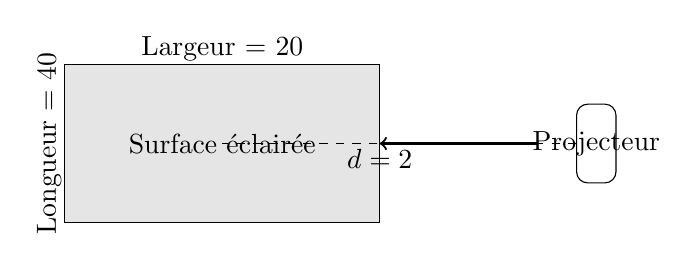
\begin{tikzpicture}
        \draw[fill=gray!20] (0,0) rectangle (4,2); % Surface éclairée
        \node at (2,1) {Surface éclairée};

        \draw[->, thick] (6, 1) -- (4,1); % Lumière du projecteur
        \draw[rounded corners] (6.5, 0.5) rectangle (7,1.5);
        \node at (6.75, 1) {Projecteur};
        
        \draw[dashed] (6.5, 1) -- (2, 1); % Distance du projecteur à la surface
        \node at (4, 0.8) {$d = \SI{2}{\meter}$};
        
        \node at (2, 2.2) {Largeur = \SI{20}{\centi\meter}};
        \node[rotate=90] at (-0.2, 1) {Longueur = \SI{40}{\centi\meter}};
    \end{tikzpicture}
\end{center}

\end{questions}

\subsection*{Question 2: IRC et commentaire}

\begin{questions}
\begin{compactitem}
    \item L’indice de rendu de couleur (IRC) est une mesure de la capacité d'une source lumineuse à restituer fidèlement les couleurs des objets par rapport à une source de référence. 
    \item Un IRC de 90, comme indiqué pour ce projecteur, signifie que la lumière produite est capable de reproduire les couleurs avec une bonne fidélité, proche de celle d'une lumière naturelle. Cela est particulièrement avantageux pour des applications artistiques où la précision des couleurs est cruciale.
\end{compactitem}
\end{questions}

\subsection*{Question 3: Calculer le flux lumineux reçu par l'écran}

\begin{questions}
Pour calculer le flux lumineux ($\Phi$) reçu par l'écran, nous utilisons la formule suivante :
\[
\Phi = E \times A
\]
où
\begin{addmargin}[4em]{1em}
\begin{compactitem}
    \item [$\Phi$] : Flux lumineux en lumens (lm)
    \item [$E$] : Éclairement en lux (lx)
    \item [$A$] : Surface éclairée en mètres carrés (\si{\meter\squared})
\end{compactitem}
\end{addmargin}

1. **Conversions dans les bonnes unités :**

   La surface de l'écran est donnée par :
   \[
   A = \text{largeur} \times \text{longueur} = \SI{0.2}{\meter} \times \SI{0.4}{\meter} = \SI{0.08}{\meter\squared}
   \]

2. **Application numérique :**

   \[
   \Phi = 500 \times 0.08 = 40
   \]

3. **Conclusion :** 

   Le flux lumineux reçu par l'écran est de \SI{40}{\lumen}.
\end{questions}

\end{solution}



\section*{Comparaison des Performances et Caractéristiques des Ampoules}

    \begin{figure}[H]
      \centering
      \includegraphics[width=0.6\linewidth]{/Users/nicolasbancel/git/education_suger/01_1ères_STD2A_pc/chap5_lumiere/a_corriger/exo_20.jpg}
      \captionsetup{labelformat=empty}
    \end{figure}

    \begin{solution}
\subsection*{Réponses aux questions}

\begin{questions}

\item \textbf{Quelle ampoule produit le plus grand flux de lumière ?}

La comparaison des flux lumineux indiqués sur les étiquettes montre que :

- \textbf{Lampodule} produit un flux lumineux de \SI{1700}{lm}.
- \textbf{Photolux} produit un flux lumineux de \SI{2300}{lm}.

Conclusion : L'ampoule \textbf{Photolux} produit le plus grand flux lumineux.

\item \textbf{Quelle ampoule possède le meilleur rendement énergétique ?}

Le rendement énergétique est souvent associé à la classe énergétique :

- \textbf{Lampodule} est classée A.
- \textbf{Photolux} est classée C.

Conclusion : L'ampoule \textbf{Lampodule} possède le meilleur rendement énergétique.

\item \textbf{Quelle ampoule donne le meilleur rendu des couleurs ?}

Le rendu des couleurs est indiqué par l'IRC (Indice de Rendu des Couleurs) :

- \textbf{Lampodule} a un IRC de 75.
- \textbf{Photolux} a un IRC de 95.

Conclusion : L'ampoule \textbf{Photolux} donne le meilleur rendu des couleurs.

\item \textbf{Quelle ampoule émet la teinte la plus chaude ?}

La température de couleur, mesurée en Kelvin (K), indique la teinte :

- \textbf{Lampodule} a une température de couleur de \SIrange{9500}{5300}{K}.
- \textbf{Photolux} a une température de couleur de \SIrange{9500}{3000}{K}.

La température de couleur la plus basse correspond à une teinte plus chaude. 

Conclusion : L'ampoule \textbf{Photolux}, avec une température de \SI{3000}{K}, émet la teinte la plus chaude.

\end{questions}
\end{solution}

\end{document}
